\documentclass[10pt]{beamer}
\usepackage[danish]{babel}
 \usepackage[utf8]{inputenc} % til at skrive æÆøØåÅ.
\usepackage{amsmath,amssymb,amsfonts,amsthm,mathrsfs,latexsym}
\usepackage{tikz,tikz-cd}
\usepackage{csquotes}
\usepackage{diagbox} % til at lave diagonal i tabelcelle
\usepackage{graphicx}% til at rette størrelsen af tabel
\usepackage{mathtools}
\usepackage{mdframed}
\usepackage{rotating}
\usepackage[matrix,arrow,ps]{xy}
\usepackage{stmaryrd}
\usepackage{tcolorbox}
\usepackage{centernot}
\newcommand*{\isoarrow}[1]{\arrow[#1,"\rotatebox{90}{\(\sim\)}"
]}
\usepackage[normalem]{ulem} % strikethrough on text: command \sout{text}
\newcommand{\indep}{\perp \!\!\! \perp}

% Beamer setup
\usetheme[style=alternative,TPlrimage=kumat2
,ku]{Frederiksberg}
\setbeamerfont{page number in head/foot}{size=\tiny}
\setbeamerfont{page number in head/foot}{size=\tiny}
\setbeamerfont{date in head/foot}{size=\tiny}
\setbeamerfont{title in head/foot}{size=\tiny}

% Titlepage
\title{Causal Inference in Dynamical Systems}
\subtitle{Convergent Cross Mapping and Alternative Approaches\\[10pt]Master's Defense}

\author[]{Rasmus Juhl Christensen\\
stud.scient.}
\institute[Faculty of Science]{Department of Mathematical Sciences}
\date[]{January 15th, 2024}

% Commands
\newcommand{\cupdot}{\mathbin{\mathaccent\cdot\cup}}

\newcommand{\mN}{\mathbb{N}}
\newcommand{\mZ}{\mathbb{Z}}
\newcommand{\mQ}{\mathbb{Q}}
\newcommand{\mR}{\mathbb{R}}
\newcommand{\mC}{\mathbb{C}}
\newcommand{\mP}{\mathbb{P}}
\newcommand{\mA}{\mathbb{A}}

\newcommand{\mF}{\mathbb{F}}

\newcommand{\mH}{\mathbb{H}}
\newcommand{\mD}{\mathbb{D}}

\newcommand{\cM}{\mathcal{M}}
\newcommand{\cH}{\mathcal{H}}
\newcommand{\cD}{\mathcal{D}}
\newcommand{\cF}{\mathcal{F}}
\newcommand{\cC}{\mathcal{C}}
\newcommand{\cSH}{\mathcal{SH}}

\newcommand{\M}{\text{M}}
\newcommand{\SL}{\text{SL}}
\newcommand{\GL}{\text{GL}}
\newcommand{\SO}{\text{SO}}
\newcommand{\PSL}{\text{PSL}}
\renewcommand{\d}{\hspace{1mm}d}
\newcommand{\p}{\partial}


\newcommand{\floor}[1]{\left\lfloor #1\right\rfloor}
\newcommand{\ceil}[1]{\left\lceil #1\right\rceil}
\newcommand{\leg}[2]{\left(\frac{#1}{#2}\right)}

\newcommand{\ths}{\hspace{0.5mm}}
\newcommand{\hs}{\hspace{1mm}}
\newcommand{\Hs}{\hspace{4mm}}
\newcommand{\HS}{\hspace{8mm}}

\newcommand{\abs}[1]{\left| #1\right|}
\newcommand{\pare}[1]{\left( #1\right)}
\newcommand{\bigPare}[1]{\bigg( #1\bigg)}
\newcommand{\cbrac}[1]{\left\{ #1\right\}}
\newcommand{\setBrac}[2]{\left\{ #1 \hs\middle|\hs #2 \right\}}
\newcommand{\brac}[1]{\left[ #1\right]}
\newcommand{\norm}[1]{\left\lVert#1\right\rVert}
\newcommand{\inProd}[1]{\left\langle#1\right\rangle}

\renewcommand{\Im}{\text{Im}\hs}
\renewcommand{\Re}{\text{Re}\hs}
\renewcommand{\phi}{\varphi}
\newcommand{\ord}{\text{ord}}
\newcommand{\supp}{\text{supp}\hs}
\newcommand{\Aut}[1]{\text{Aut}(#1)}
\newcommand{\stab}[2]{\text{Stab}_{#1}\pare{#2}}
\newcommand{\cusp}[1]{\text{Cusps}\pare{#1}}
\newcommand{\dist}[1]{\text{dist}\pare{#1}}

\newcommand{\nl}{\newline \\}
\DeclareMathOperator{\chara}{char}
\DeclareMathOperator{\Gal}{Gal}
\DeclareMathOperator{\End}{End}

\DeclareMathOperator{\Tr}{Tr}

\begin{document}
\frame[plain]{\titlepage}


\begin{frame}{Program}
\onslide<1->{
10.30-11.00: A presentation on the following topics:
\begin{enumerate}
	\item Time Series
	\item Stochastic Models
	\item Granger Causality
	\item Dynamical Models
	\item Takens' Theorem
	\item Convergent Cross Mapping
	\item Extensions
\end{enumerate}}
11.00: Questions.
\end{frame}

\begin{frame}{Time Series}
Consider the following example:
\onslide<1->{
\begin{center}
	\begin{figure}[!ht]
		\includegraphics[width=\textwidth]{{"../../r code/sardine"}.png}
	\end{figure}
\end{center}
}

\end{frame}


\begin{frame}{Time Series Characteristics}We imagine the following generical set-up in this presentation:
\begin{align*}
X_1,\ldots, X_T\\
Y_1,\ldots, Y_T\\
Z_1,\ldots, Z_T
\end{align*}
We consider thus the following features of our models:
\begin{itemize}
	\item<2-> Dependence over time
	\item<3-> Randomness or unpredictability
	\item<4-> Interference - what happens when we \enquote{push} a variable?
\end{itemize}
\onslide<5->{
The key: building a model. In this presentation, we will introduce and compare two settings:}
\begin{itemize}
	\item<6-> Stochastic model - randomness coming from noise,
	\item<7-> Dynamical model - randomness coming from chaos.
\end{itemize}
\onslide<8->{
$\longrightarrow $ identifiability from lagged information.}
\end{frame}

\begin{frame}{Stochastic Models}
We get the randomness in stochastic models via noise terms. For each variable, we will model as follows:
$$X_t=f(\underbrace{X_{t-1}}_{\text{last state}},\underbrace{\ldots\ldots\ldots\ldots\ldots}_{\text{additional information}},\underbrace{u^X_t}_{\text{noise}})$$
\onslide<2->{
For instance, one could imagine the following situation:
\begin{align*}
X_t&=f_X(X_{t-1}, Z_{t-1}, u^X_t)\\
Y_t&=f_Y(Y_{t-1}, Z_{t-1},u^Y_t)\\
Z_t&=f_Z(Z_{t-1}, u^Z_t)
\end{align*}
}
\onslide<3->{
Causality: 
\begin{itemize}
\item<3-> \enquote{Changes in the cause will result in changes in the effect}.
\item<4-> In this example: $Z$ \textit{causes} $X$ and $Y$. 
\item<5-> Reformulated in terms of Granger causality: 
$$X_t\centernot\indep Z_{t-1}\mid (X_{t-1},Y_{t-1})$$
\end{itemize}
}
\end{frame}

\begin{frame}{Dynamical Models}
We get the randomness in dynamical models via chaos. We move to continuous setting:
$$\frac{dX_t}{dt}=f(\underbrace{X_t}_{\text{current state}},\underbrace{\ldots\ldots\ldots\ldots\ldots}_{\text{additional information}})$$
\onslide<2->{
\noindent\textbf{Completely deterministic!\\[10pt]}
}
\onslide<3->{
For instance, one could imagine the following situation:
\begin{align*}
\frac{dX_t}{dt}=f_X(X_t, Z_t),\quad \frac{dY_t}{dt}=f_Y(Y_t, Z_t),\quad \frac{dZ_t}{dt}=f_Z(Z_t)
\end{align*}
}
\onslide<4->{
Causality: 
\begin{itemize}
\item<4-> \enquote{Changes in the cause will result in changes in the effect}.
\item<5-> In this example: $Z$ \textit{causes} $X$ and $Y$. 
\item<6-> How do we detect it?
\end{itemize}
}
\end{frame}

\begin{frame}{Chaotic Attractors}
Meteorologist Edward Lorenz at MIT modelled atmospheric convection, and discovered the Lorenz system in 1963:
\begin{align*}
\frac{dX_t}{dt}&=\sigma(Y_t-X_t),\quad \frac{dY_t}{dt}=-X_tZ_t+rX_t-Y_t,\\
\frac{dZ_t}{dt}&=X_tY_t-bZ_t
\end{align*}
\onslide<2->{
Result: a butterfly!
\begin{center}
	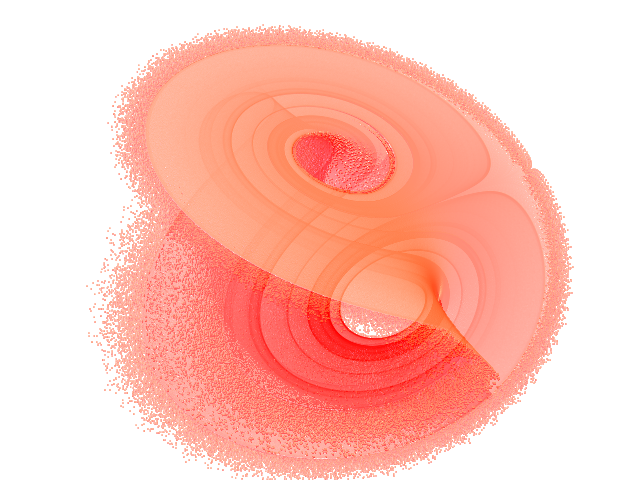
\includegraphics[scale=0.25]{"../../tex/lorenz.png"}
\end{center}
}
\end{frame}

\begin{frame}{State Space Reconstruction}
Strange behavior! 
\begin{itemize}
\item<2-> Geometric object: a surface!
\item<3-> Strong sensitivity to starting conditions.
\item<4-> Dense trajectories.
\end{itemize}
\only<5-6>{
A resulting time series becomes:
\begin{center}
	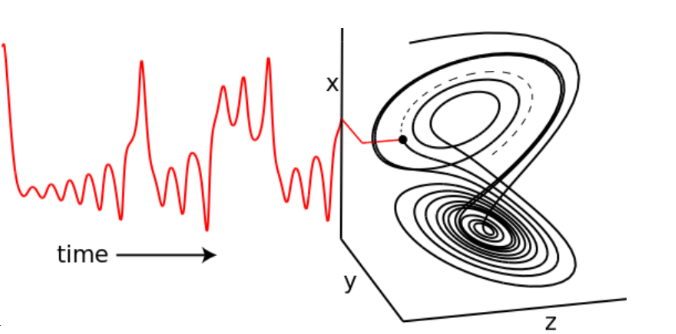
\includegraphics[scale=0.38]{Lorenz.png}
\end{center}
}
\only<6-6>{
\begin{center}
	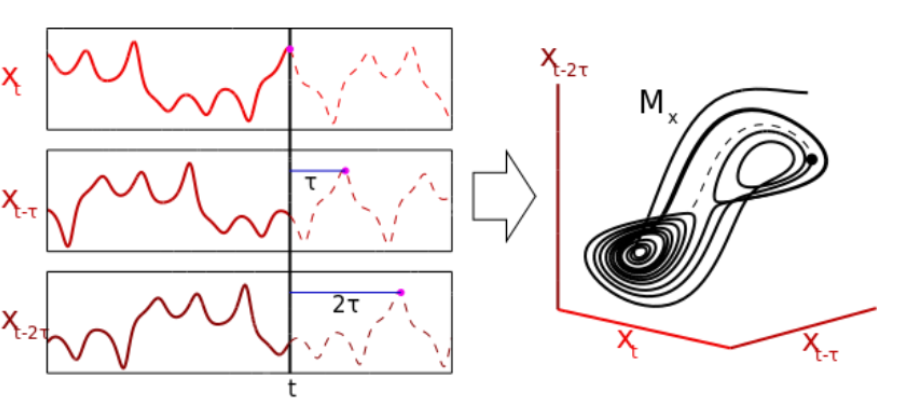
\includegraphics[scale=0.38]{Lorenz2.png}
\end{center}
}
\onslide<7->{
A resulting time series becomes:
 \begin{center}
	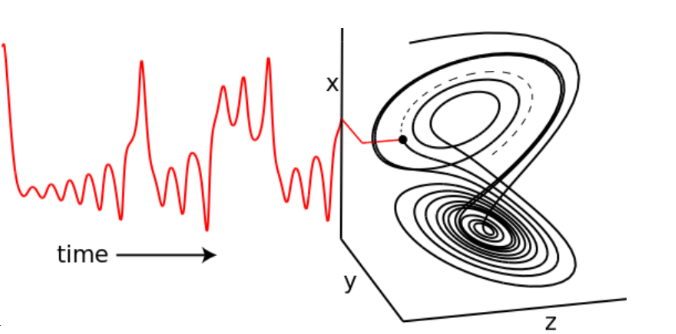
\includegraphics[scale=0.38]{Lorenz.png}
\end{center}
 \begin{minipage}[c]{0.6\textwidth}
    	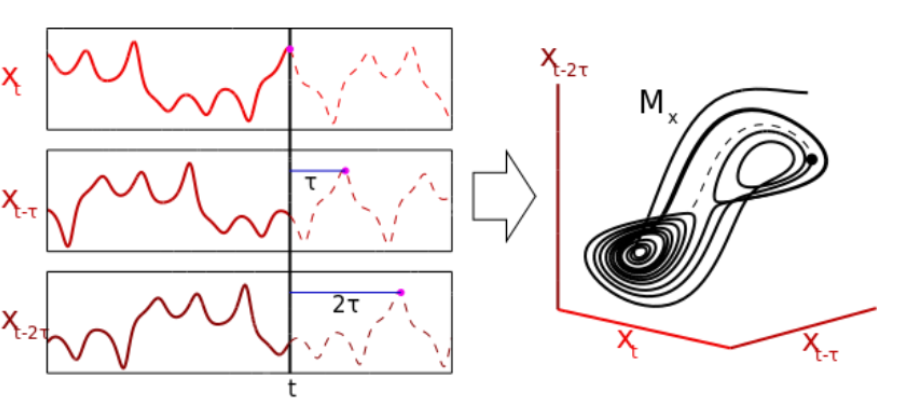
\includegraphics[scale=0.38]{Lorenz2.png}
  \end{minipage} \hfill
   \begin{minipage}[c]{0.3\textwidth}
  \begin{mdframed}[innerleftmargin=0pt, innerrightmargin=0pt, innertopmargin=0pt, innerbottommargin=5pt, linewidth=1pt]
    \begin{align*}
      \frac{dX_t}{dt}&=f_X(X_t, Z_t) \\
      \frac{dY_t}{dt}&=f_Y(Y_t, Z_t) \\
      \frac{dZ_t}{dt}&=f_Z(Z_t)
    \end{align*}
  \end{mdframed}
    \end{minipage}
  
}

\end{frame}
\begin{frame}{Causal Inference}
Takens' theorem:
\begin{align*}
(X_t,Y_t,Z_t)\mapsto \left(X_t,X_{t-\tau},\ldots,X_{t-4\tau}\right)
\end{align*}
is an \textit{embedding} of the attractor \textit{generically}. In particular,
\begin{itemize}
\item<2-> if there is no causal link from $Z$ or $Y$ to $X$, then Takens' theorem does \textit{not} hold!
\item<3-> if there is a causal link from from $Z$ to $X$ and $Y$ to $X$, then we can \textit{hope} Takens' theorem does hold. 
\item<4-> we can hope to recover a system consisting of \textit{all} causes of a variable \textit{in principle}.
\end{itemize}
\onslide<5->{
Key ingredients:
\begin{itemize}
\item<6-> Causal model consisting of functional assignments in ODE's.
\item<7-> Emergence of geometric structure from solutions.
\item<8-> Decomposition of geometry according to causal structure.
\end{itemize}
}
\end{frame}

\begin{frame}{Convergent Cross Mapping}
In practice, we start for a fixed number of points by computing the state space reconstructions or \textit{shadow manifolds} $M_X, M_Y$ and $M_Z$.\\[5pt]
\onslide<2->{
To compute the cross-mapping skill from say $X$ to $Y$, we proceed as follows:
\begin{enumerate}
	\item<3-> At time $t$, we consider $x_t=(X_t,X_{t-\tau},\ldots,X_{t-E\tau})\in M_X$.
	\item<4-> We locate the closest points on $M_X$ of $x_t$, and denote their time stamps $t_1,\ldots, t_{E+1}$.
	\item<5-> We compute the estimate 
	$$\hat{Y}_t|M_X=\sum_{i=1}^{E+1} \frac{u_i}{\sum_{i=1}^{E+1} u_j} Y_{t_i}$$
	with $u_i=\exp\left(-\frac{\norm{x(t)-x(t_i)}}{\norm{x(t)-x(t_1)}}\right)$. 
\end{enumerate}

}
\onslide<6->{
We compute the cross-mapping skill as the correlation between $\hat{Y}_t|M_X$ and $Y_t$. 
}

\end{frame}
\begin{frame}{Convergent Cross Mapping pt. 2}
Visualization:
\begin{center}
	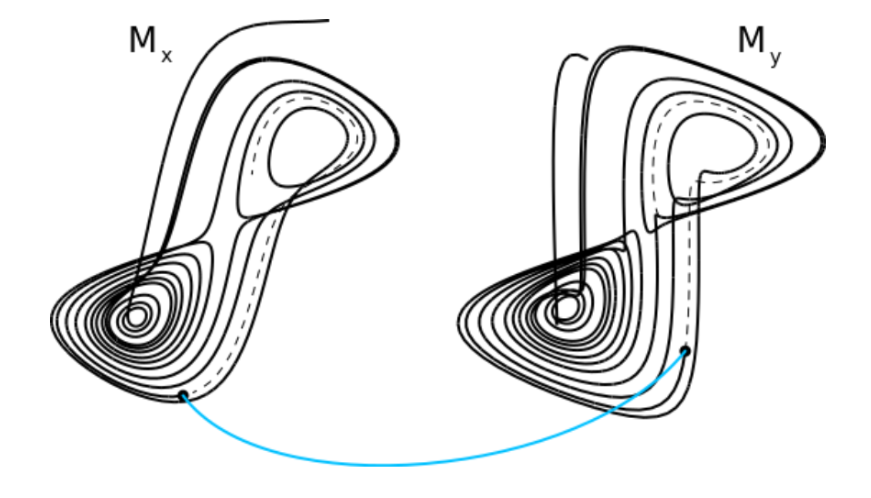
\includegraphics[scale=0.3]{Lorenz3.png}
	\end{center}
\only<2-2>{
In practice (no transformation!) with $\tau=1$, $E=4$:\\
\begin{minipage}[c]{0.45\textwidth}
    	\includegraphics[scale=0.3]{{"../../r code/p1"}.png}
  \end{minipage} \hfill
   \begin{minipage}[c]{0.45\textwidth}
    	\includegraphics[scale=0.3]{{"../../r code/p2"}.png}
  \end{minipage}
}

\onslide<3->{
In practice (no transformation!) with $\tau=2$, $E=4$:\\
\begin{minipage}[c]{0.45\textwidth}
    	\includegraphics[scale=0.3]{{"../../r code/p3"}.png}
  \end{minipage} \hfill
   \begin{minipage}[c]{0.45\textwidth}
    	\includegraphics[scale=0.3]{{"../../r code/p4"}.png}
  \end{minipage}
}

\end{frame}


\begin{frame}{Comparison of Models}
In both settings, we share the modelling approach:
\begin{itemize}
	\item<2-> Functional assignments based on graph structure.
	\item<3-> Modularity assumption on interventions.
\end{itemize}
\onslide<4->{
However, there are two properties that distinguish these models:
\begin{itemize}
	\item<5-> Non-separability of information.
	\item<6-> Deterministic non-linear dynamics.
\end{itemize}
}
\onslide<7->{
Advantages of convergent cross mapping:
\begin{itemize}
	\item<8-> We do not need to observe all variables of interest.
	\item<9-> We do not need to assume much about the functional expressions.*
\end{itemize}
}
\onslide<10->{
Disadvantages of convergent cross mapping:
\begin{itemize}
	\item<11-> No model formulated that explicitly satisfies all technical assumptions.
	\item<12-> Problems in face of synchronicity and noise.
	\item<13-> Regime dependence.
\end{itemize}
}
\end{frame}


\begin{frame}{Future Work}
The following ideas was considered, but not fully developed:
\begin{enumerate}
	\item<2-> Give a full description of a model satisfying the theoretical guarantees.
	\item<3-> We can imagine that we observe 
	$$X_t+\varepsilon_t^X$$
	with some observation noise $X_t$. 
	\item<4-> We can imagine 
	$$\frac{dX_t}{dt}=f(X_t,X_{t-\tau},Y_t,\ldots)$$
	\item<5-> Alternative, we can imagine an SDE
	$$dX_t=f(X_{t-},Y_{t-},\ldots) dZ_t$$
	\item<6-> The link between limiting distributions and attractor sets.
\end{enumerate}
\end{frame}



\begin{frame}{Questions}

\end{frame}




\end{document}
